% \clearpage
\section{Method}

	The algorithm that will be used is the finite-size Density Matrix Renormalization Group (DRMG) with $2$-site update. It follows almost to the letter the method described in \cite{schollwoeck2011}.

	Everything will be coded in python language, from scratch, except for 
	\begin{itemize}
		\item the contraction of tensors for which a very convenient function called \verb_ncon_ \cite{pfeifer2015} for python will be used, which wraps the \verb_numpy.tensordot_ into an intuitive way.
		\item the SVD routine for which \verb_numpy.linalg.svd_ will be used.
		\item the diagonalization routine of the effective Hamiltonian whenever it requires excitation energies to be found for which ARPACK \cite{lehoucq1998} implemented in \verb_scipy.sparse.linalg.eigen.arpack_ will be used.
	\end{itemize}

	\subsection{Brief recall on DMRG}

        The finite-size DMRG is summarized in \eqref{eq:dmrgSum}. The growth process of \emph{eg} block $B$ is done at the expense of block $A$, which shrinks \emph{ie} old shorter blocks $A$ are reused. This is continued until $A$ is so small as to have a complete Hilbert space. Then the growth direction is reversed. $A$ grows at the expense of $B$, including new ground state determinations and basis choices for $A$, until $B$ is small enough to have a complete Hilbert space, which leads to yet another reversal of growth direction. This sweeping through the system is continued until energy converges. The intuitive motivation for this procedure is that after each sweep, blocks $A$ or $B$ are determined in the presence of an ever improved embedding.
        
        The ground state can be found using an iterative method by minimizing the energy $E = \frac{\ev{\mc H}{\psi}}{\braket{\psi}}$ thus finding
        \be \min_{\ket \psi, \lambda} \ev{\mc H}{\psi} - \lambda\braket{\psi} \ee
        The problem is that if one considers all the matrices $M$, the problem is highly non-linear. But one can proceed by keeping all the matrices on the sites except the one considered fixed. Of course, this is computationally worth --- quadratic form --- but not optimal. To calculate the terms of the minimization, note that it can be recast into a generalized eigenvalue problem
        \be \mc H v - \lambda \mc N v =0 \ee
        with $v_{\sigma_\ell,a_{\ell-1},a_\ell} = M^{\sigma_\ell}_{a_{\ell-1},a_\ell}$. If $\ket\psi$ is mixed canonical, thus left-normalized at the left of the site $\ell$ and right-normalized on the right, then $\mc N = \mathbb 1$, so that the problem reduces to a standard eigenvalue problem.

        The algorithm is as follows
        \begin{itemize}
            \item start for a random $\ket \psi$ made of the matrices $M^{\sigma_\ell}$
            \item right-normalize it, \emph{ie} write it a product a right-orthonormal matrices $B^{\sigma_\ell}$ 
            \item run the optimization from $\ell=1$ to $L-1$, that is, solve the eigenvalue problem for $M^{\sigma_\ell}$, then left-normalize it to $A^{\sigma_\ell}$ by SVD, absorb the $SV^\dagger$ into the $M^{\sigma_{\ell+1}}$, then move to the $\ell+1$ site and repeat until $L-1$
            \item start from $\ell = L$ to 2, and do the same but right-normalizing
            \item repeat the sweeps until convergence, but can fall in local minimum thus seek for the null error on the energy
        \end{itemize}

        \be \begin{split} &M_0 B_0 B_0 B_0 \cdots B_0 \\ \xrightarrow{\text{optimize}} &M_1 B_0 B_0 B_0 \cdots B_0 \xrightarrow{\text{SVD}} A_1 M_0 B_0 B_0 \cdots B_0 \\ \xrightarrow{\text{optimize}} &A_1 M_1 B_0 B_0 \cdots B_0 \xrightarrow{\text{SVD}} A_1 A_1 M_0 B_0 \cdots B_0 \\ \xrightarrow{\text{optimize}} &A_1 A_1 M_1 B_0 \cdots B_0 \xrightarrow{\text{SVD}} A_1 A_1 A_1 M_0 \cdots B_0 \\ \xrightarrow{\cdots} &A_1 A_1 A_1 A_1 \cdots M_0 \\ \xrightarrow{\text{optimize}}  &A_1 A_1 A_1 A_1 \cdots M_1 \xrightarrow{\text{SVD}} A_1 A_1 A_1 A_1 \cdots B_1 \\ \xrightarrow{\cdots} &A_1 A_1 A_1 M_1 \cdots B_1 \\ \xrightarrow{\text{optimize}} &A_1 A_1 A_1 M_2 \cdots B_1 \xrightarrow{\text{SVD}} A_1 A_1 M_1 B_2 \cdots B_1 \\ \xrightarrow{\text{optimize}} &A_1 A_1 M_2 B_2 \cdots B_1 \xrightarrow{\text{SVD}} A_1 M_1 B_2 B_2 \cdots B_1 \\ \xrightarrow{\text{optimize}} &A_1 M_2 B_2 B_2 \cdots B_1 \xrightarrow{\text{SVD}} M_1 B_2 B_2 B_2 \cdots B_1 \\ \xrightarrow{\cdots} & \end{split} \label{eq:dmrgSum} \ee

	\subsection{MPO construction for OBCs and free at both edges}
		
		Here, the open boundary conditions (OBCs) with states at both edges of the chain, denoted as $[ff]$ will be of interest.

		For simplicity, since in OF model \eqref{eq:OF} there is the critical $J=h$ TFI model \eqref{eq:TFI}, the former will be slightly modified by adding the $J$ and $h$ couplings appearing in TFI to only make use of one MPO that allows to switch between the different model just by tuning the different coefficients. The Hamiltonian is therefore
		\be \mc H = - 2\lambda_I \sum_j [J\sigma^x_j \sigma^x_{j+1} + h\sigma^z_j] + \lambda_3 \sum_j [\sigma^z_j\sigma^x_{j+1}\sigma^x_{j+2} + \sigma^x_j\sigma^x_{j+1}\sigma^z_{j+2}] + \lambda_c \sum_j [\sigma^x_j\sigma^y_{j+1} - \sigma^y_j\sigma^y_{j+1}] \label{eq:modifiedOF} \ee

		To construct the MPO representing \eqref{eq:modifiedOF} in the bulk, only consider one term in the sum over $j$, namely $j=\ell$. Looking at the string of operators from its right end, the action of each operator on each bond moves the string into a new state, whose label correspond to the string of operators on the right of the bond considered. Then the typical action of the term $l$ is viewed as
		\be \arraycolsep=1.5pt \begin{array}{llclclcll}
			\cdots &\one \stackrel{7}{\otimes} \one \stackrel{7}{\otimes} &-2\lambda_I h \sigma^z &\stackrel{1}{\otimes} &\one &\stackrel{1}{\otimes} &\one &\stackrel{1}{\otimes} \one &\cdots \\
			\cdots &\one \stackrel{7}{\otimes} \one \stackrel{7}{\otimes} &-2\lambda_I J \sigma^x &\stackrel{2}{\otimes} &\sigma^x &\stackrel{1}{\otimes} &\one &\stackrel{1}{\otimes} \one &\cdots \\
			\cdots &\one \stackrel{7}{\otimes} \one \stackrel{7}{\otimes} &\lambda_3 \sigma^z &\stackrel{4}{\otimes} &\sigma^x &\stackrel{2}{\otimes} &\sigma^x &\stackrel{1}{\otimes} \one &\cdots \\
			\cdots &\one \stackrel{7}{\otimes} \one \stackrel{7}{\otimes} &\lambda_3 \sigma^x &\stackrel{5}{\otimes} &\sigma^x &\stackrel{3}{\otimes} &\sigma^z &\stackrel{1}{\otimes} \one &\cdots \\
			\cdots &\one \stackrel{7}{\otimes} \one \stackrel{7}{\otimes} &\lambda_c \sigma^x &\stackrel{6}{\otimes} &\sigma^y &\stackrel{1}{\otimes} &\one &\stackrel{1}{\otimes} \one &\cdots \\
			\cdots &\one \stackrel{7}{\otimes} \one \stackrel{7}{\otimes} &\lambda_c \sigma^y &\stackrel{2}{\otimes} &\sigma^x &\stackrel{1}{\otimes} &\one &\stackrel{1}{\otimes} \one &\cdots
		\end{array} \ee
		where the states have been labeled following \autoref{tab:statesOF}.

		\begin{table}[h!]
			\centering
			\begin{tabular}{lcl}
				\hline
				1 & --- & $\one$ \\
				2 & --- & $\sigma^x$ \\
				3 & --- & $\sigma^z$ \\
				4 & --- & $\sigma^x \otimes \sigma^x$ \\
				5 & --- & $\sigma^x \otimes \sigma^z$ \\
				6 & --- & $\sigma^y$ \\
				7 & --- & completed interaction \\
				\hline
			\end{tabular}
			\caption{Labeling of states involved in the construction of the MPO for the \eqref{eq:modifiedOF} Hamiltonian with open $[ff]$ BCs. Each term corresponds to what is on the right of the bond considered.}
			\label{tab:statesOF}
		\end{table}
		This is encoded in the bulk matrix of the MPO, called $W^{[\ell]}$, whose entries $W_{ij}^{[\ell]}$ correspond to the operator making the transition from the state $j \to i$. The bulk matrix for the Hamiltonian \eqref{eq:modifiedOF} is therefore the $7\times 7$ matrix
		\be W^{[\ell]} = \bmqty{
			\one & \cdot & \cdot & \cdot & \cdot & \cdot & \cdot \\
			\sigma^x & \cdot & \cdot & \cdot & \cdot & \cdot & \cdot \\
			\sigma^z & \cdot & \cdot & \cdot & \cdot & \cdot & \cdot \\
			\cdot & \sigma^x & \cdot & \cdot & \cdot & \cdot & \cdot \\
			\cdot & \cdot & \sigma^x & \cdot & \cdot & \cdot & \cdot \\
			\sigma^y & \cdot & \cdot & \cdot & \cdot & \cdot & \cdot \\
			-2\lambda_I h \sigma^z & -2\lambda_I J \sigma^x - \lambda_c \sigma^y & \cdot & \lambda_3 \sigma^z & \lambda_3 \sigma^x & \lambda_c \sigma^x & \one
			} \ee
		Finally, it remains to find the $W^{[1]}$ and $W^{[L]}$ matrices. This is easily done by noticing that $W^{[1]}$ only enables to complete the unfinished interactions started with $W^{[2]}$ and $W^{[3]}$, then is equal to last row of $W^{[\ell]}$. Similarly, $W^{[L]}$ only serves as a starter of interactions that will be completed with $W^{[L-1]}$ and $W^{[L-2]}$, then is equal to the first column of $W^{[\ell]}$. In the end, they are written
		\be W^{[1]} = \bmqty{-2\lambda_I h \sigma^z \\ -2\lambda_I J \sigma^x - \lambda_c \sigma^y \\ \cdot \\ \lambda_3 \sigma^z \\ \lambda_3 \sigma^x \\ \lambda_c \sigma^x \\ \one}^\top \qq{and} W^{[L]} = \bmqty{\one \\ \sigma^x \\ \sigma^z \\ \cdot \\ \cdot \\ \sigma^y \\ -2\lambda_I h \sigma^z} \ee

	\subsection{MPO construction for OBCs with pinning}
		
		The model presented with $[ff]$ BCs can suffer from entanglement coming from the edge states. Hence, it can be useful to fix their spin. For that purpose, the notation which will be used to denote the BCs is presented on \autoref{tab:pinningBCs}. Moreover, even if everything is expressed in the $z$-basis, the spins will be fixed in the $x$-direction since the TFI \eqref{eq:TFI} is $\mathbb Z_2$-symmetric with respect to flipping all the spins in the $x$-direction. Then the states $\ket \pm$ are introduced as
		\be \sigma^x \ket\pm = \pm \ket \pm \label{eq:xPinDef} \ee
		where $\ket +$ means the spin pointing up and $\ket -$ pointing down in $x$-direction.

		\begin{table}[h!]
			\centering
			\begin{tabular}{rcl}
				\hline
				$[ff]$ & $\sim$ & free at both ends \\
				$[f\pm]$ & $\sim$ & free at left end and $\ket \pm_\text{right}$\\
				$[f\pm]$ & $\sim$ & $\ket \pm_\text{left}$ and free at right end  \\
				$[\pm \pm]$ & $\sim$ & $\ket \pm_\text{left}$ and $\ket \pm_\text{right}$ \\
				\hline
			\end{tabular}
			\caption{Labeling of the different BCs used with the definition of the states in \eqref{eq:xPinDef}.}
			\label{tab:pinningBCs}
		\end{table}

		To fix a spin on a site, it suffices to introduce a pinning field $h_\text{pin}$ in the direction wanted. Therefore, the term $h_\text{pin} \sigma^x$ is added in the Hamiltonian MPO as 
		\be W^{[1]} = \bmqty{-2\lambda_I h \sigma^z {\color{magenta}+h_\text{pin}\sigma^x} \\ -2\lambda_I J \sigma^x - \lambda_c \sigma^y \\ \cdot \\ \lambda_3 \sigma^z \\ \lambda_3 \sigma^x \\ \lambda_c \sigma^x \\ \one}^\top \qq{and} W^{[L]} = \bmqty{\one \\ \sigma^x \\ \sigma^z \\ \cdot \\ \cdot \\ \sigma^y \\ -2\lambda_I h \sigma^z {\color{magenta}+h_\text{pin}\sigma^x}} \ee
		where the bulk $W^{[l]}$, $l\in]1, L[$ remain the same.

	\subsection{MPO construction for PBCs}

		It will be useful to use DMRG with an Hamiltonian with periodic boundary conditions (PBCs). This would remove the edge states that would be present in the free OBCs and might still be in the fixed OBCs. However, PBCs DMRG in the MPS formalism suffers from problems \cite{schollwoeck2011}, and several ideas have been put on the stage to cope with them \cite{dey2016, pippan2010, verstraete2004, pirvu2011}, and the main issue that arises when the goal is not to drastically change the way the DMRG was coded, is that to get the same precision on the targeted ground state with OBCs and PBCs, the bond dimension $\chi$ in OBCs has to be increased to $\chi^2$ in PBCs \cite{schollwoeck2011}. Nonetheless, these issues will not be taken into account here, but the the generalized eigenvalue problem arising from naively taking the trace of the MPS to represent PBCs will be solved by folding the MPS as in \autoref{fig:foldMPS}.

		\begin{figure}[h!]
			\centering
			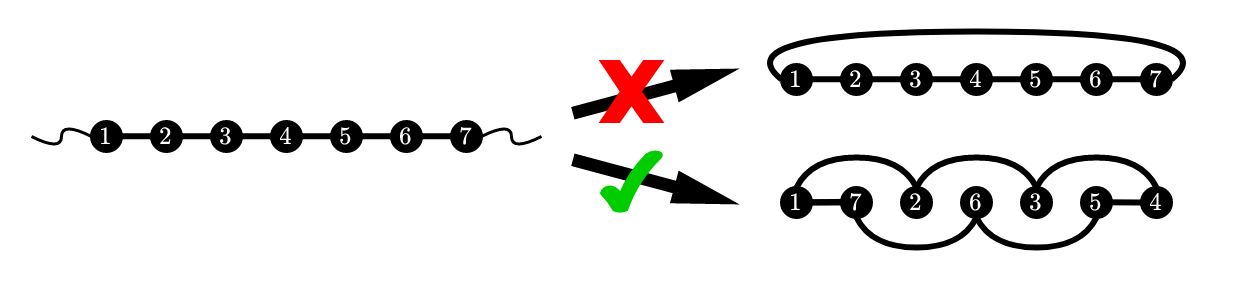
\includegraphics[scale=0.4]{../images/pbcmps.png}
			\caption{Way to represent the MPS in OBCs and its extension to PBCs, where nearest-neighbor couplings become second-nearest-neighbor ones, here presented with 7 sites.}
			\label{fig:foldMPS}
		\end{figure}

		This way to represent the MPS only amounts to change the MPO used. However, one must be very careful when deriving it, as many of the terms in \eqref{eq:OF} appearing at the edges change in a non trivial way. Noticing that $\lambda_c=0$ will be taken to simplify here, the bulk is becoming the $15\times15$ matrix
		\be W^{[\ell]} = \bmqty{
			\one & \cdot & \cdot & \cdot & \cdot & \cdot & \cdot & \cdot & \cdot & \cdot & \cdot & \cdot & \cdot & \cdot & \cdot \\
			\sigma^x & \cdot & \cdot & \cdot & \cdot & \cdot & \cdot & \cdot & \cdot & \cdot & \cdot & \cdot & \cdot & \cdot & \cdot \\
			\sigma^z & \cdot & \cdot & \cdot & \cdot & \cdot & \cdot & \cdot & \cdot & \cdot & \cdot & \cdot & \cdot & \cdot & \cdot \\
			\cdot & \one & \cdot & \cdot & \cdot & \cdot & \cdot & \cdot & \cdot & \cdot & \cdot & \cdot & \cdot & \cdot & \cdot \\
			\cdot & \cdot & \one & \cdot & \cdot & \cdot & \cdot & \cdot & \cdot & \cdot & \cdot & \cdot & \cdot & \cdot & \cdot \\
			\cdot & \cdot & \cdot & \cdot & \cdot & \cdot & \cdot & \cdot & \cdot & \cdot & \cdot & \cdot & \cdot & \cdot & \cdot \\
			\cdot & \cdot & \cdot & \cdot & \cdot & \cdot & \cdot & \cdot & \cdot & \cdot & \cdot & \cdot & \cdot & \cdot & \cdot \\
			\cdot & \cdot & \cdot & \sigma^x & \cdot & \cdot & \cdot & \cdot & \cdot & \cdot & \cdot & \cdot & \cdot & \cdot & \cdot \\
			\cdot & \cdot & \cdot & \cdot & \sigma^x & \cdot & \cdot & \cdot & \cdot & \cdot & \cdot & \cdot & \cdot & \cdot & \cdot \\
			\cdot & \cdot & \cdot & \cdot & \cdot & \cdot & \cdot & \cdot & \cdot & \cdot & \cdot & \cdot & \cdot & \cdot & \cdot \\
			\cdot & \cdot & \cdot & \cdot & \cdot & \cdot & \cdot & \cdot & \cdot & \cdot & \cdot & \cdot & \cdot & \cdot & \cdot \\
			\cdot & \cdot & \cdot & \cdot & \cdot & \cdot & \cdot & \one & \cdot & \cdot & \cdot & \cdot & \cdot & \cdot & \cdot \\
			\cdot & \cdot & \cdot & \cdot & \cdot & \cdot & \cdot & \cdot & \one & \cdot & \cdot & \cdot & \cdot & \cdot & \cdot \\
			\cdot & \cdot & \cdot & \cdot & \cdot & \cdot & \cdot & \cdot & \cdot & \cdot & \cdot & \cdot & \cdot & \cdot & \cdot \\
			-2\lambda_I h \sigma^z & \cdot & \cdot & -2\lambda_I J \sigma^x & \cdot & \cdot & \cdot & \cdot & \cdot & \cdot & \cdot & \lambda_3 \sigma^z & \lambda_3 \sigma^x & \cdot & \one} \ee
		Now, there are numerous changes to make for the matrices on sites near the boundaries, that are summarized in \autoref{tab:mpoPBCsBoundaries}, where PBCs and antiperiodic boundary conditions (aPBCs) are also given, noticing that aPBCs amount to a change
		\be \sigma^x_L \sigma^x_1 \to - \sigma^x_L \sigma^x_1 \ee

		\begin{table}[h!]
			\centering
			\begin{tabular}{c|lllll}
				$l$ & \multicolumn{1}{c}{$1$} &\multicolumn{1}{c}{$2$} & \multicolumn{1}{c}{$L-3$} & \multicolumn{1}{c}{$L-2$} & \multicolumn{1}{c}{$L-1$} \\
				\hline
				\multirow{5}{*}{$W_{ij}^{[l]}$ with $(i,j)$} & $(2, 15)$ : $\mp 2\lambda_I J \sigma^x$ & $(2, 14)$ : $\sigma^z$ & $(10, 15)$ : $\lambda_3 \sigma^z$ & $(6, 10)$ : $\one$ & $(2, 6)$ : $\sigma^x$ \\
				& $(7, 15)$ : $\pm \lambda_3 \sigma^x$ & $(3, 7)$ : $\sigma^x$ & $(11, 15)$ : $\lambda_3 \sigma^x$ & $(6, 15)$ : $\lambda_3 \sigma^z$ & $(2, 14)$ : $\sigma^z$ \\
				& $(8, 15)$ : $\lambda_3 \sigma^z$ & & & $(7, 11)$ : $\one$ & $(2, 15)$ : $-2\lambda_I J \sigma^x$ \\
				& $(9, 15)$ : $\pm \lambda_3 \sigma^x$ & & & $(14, 15)$ : $\lambda_3 \sigma^x$ & $(3, 7)$ : $\sigma^x$ \\
				& $(14, 15)$ : $\lambda_3 \sigma^x$ & & & & \\
			\end{tabular}
			\caption{All changes made in the matrices of the MPO for Hamiltonian \eqref{eq:OF} with $\lambda_c=0$ for PBCs and aPBCS respectively.}
			\label{tab:mpoPBCsBoundaries}
		\end{table}
		Finally, once again, $W^{[1]}$ is actually taken to be the last row of $W^{[1]}$ and $W^{[L]}$ the first column of $W^{[L]}$.

	\subsection{Excitation energies}

		DRMG is particularly suited to find the ground state of an Hamiltonian associated to its lowest eigenvalue. However, it is often useful to find the excitation spectrum of the Hamiltonian, or at least its low-lying excitation energies. To this end, one can exploit the property of DRMG to finding the ground state and use an Hamiltonian slightly modified so that the state having a vanishing overlap with the ground state is punished with a large energy, allowing to converge to the state orthogonal to the ground state with the same or higher energy. To be specific, a first DRMG can be run converging to the ground state $\ket{\psi_0}$ of $\mc H$. Then a new DRMG is run with
		\be \tilde{\mc H} = \mc H + \lambda_0 \dyad{\psi_0} \ee 
		with $\lambda_0 > |E_1-E_0|$. One can repeat this procedure to find the $n$ excited states of $\mc H$ by applying
		\be \tilde{\mc H} = \mc H + \sum_{i=0}^{n-1} \lambda_i \dyad{\psi_i} \ee
		with $\ket{\psi_i}$ the ground state of the $i^\text{th}$ run of DMRG, that must correspond to the $i^\text{th}$ excited state. This procedure however need to run $n+1$ DRMG simulations to find the $n^\text{th}$ excited state.

		Sometimes, only the excitation energies are needed. Hence, there is no point to finding the states associated. To this end, it is possible to find and store the excitation energies find in the diagonalization of the effective Hamiltonian in the $2$-site update \cite{chepiga2017}. This is done using \emph{eg} Implicitly Restarted Arnoldi Method that has an implementation in ARPACK software \cite{lehoucq1998}. This method works incredibly well in critical systems but struggles in gapped systems \cite{chepiga2017}.

	\subsection{Parity}

		The Hamiltonian \eqref{eq:OF} with $\lambda_c=0$ is $\mathbb Z_2$-symmetric commuting with the unitary spin-flip operator $\mc F$ defined as
		\be \mc F \equiv \prod_j \sigma^z_j \ee
		which also called the fermion-number parity. Moreover, $\mc F^2 =1$, meaning $\mc H$ is divided into sectors corresponding to the eigenvalues $\pm$ of $\mc F$. It is called the spin-flip since it flip all the spins along the $x$-direction as it can be seen from
		\be \begin{split} \sigma^z \ket \pm &= \frac{1}{\sqrt 2} \sigma^z [\ket \uparrow \pm \ket \downarrow] = \frac{1}{\sqrt 2} [\ket \uparrow \mp \ket \downarrow] \\ &= \ket \mp \end{split} \ee
		where $\ket \uparrow$ and $\ket \downarrow$ are the spin up and down in the $z$-direction. This parity operator will be useful to compute ratios of energies deriving from conformal dimension of operators at the critical points described by a CFT. 

		To implement it in the DRMG, notice that the goal is to find the ground state in a sector of $\mc H$. Thus it is useful to defined the projectors
		\be \mc F^\pm = \frac 1 2 [\one \pm \mc F] \ee
		that project the states to which it is applied on the ones with corresponding eigenvalue $\pm$ of $\mc F$. In the MPO formalism, $\mc F^\pm$ is simply given by
		\be W^{[\ell]} = \bmqty{\one & \cdot \\ \cdot & \sigma^z} \ee
		with the boundary matrices
		\be W^{[1]} = \frac 1 2 \bmqty{\one \\ \pm \sigma^z}^\top \qq{and} W^{[L]} = \bmqty{\one \\ \sigma^z} \ee
		Now, the only thing to do is to apply the new Hamiltonian $\tilde{\mc H}^\pm$ in the MPO form to the chain in the DMRG, where 
		\be \tilde{\mc H}^\pm = \mc F^\pm \mc H \mc F^\pm \ee
		to find the ground state of $\mc H$ in the sector with eigenvalue $\pm$ of $\mc F$.

	\subsection{Central charge}

		One of the main thing that can be done to characterize of critical models described by a CFT is to compute the central charge from the entanglement entropy. DMRG under MPS formalism is particularly well suited since the entanglement entropy on each bond is computed from the singular values on that bond. The formulas that will be used will be called for convenience the Cardy-Calabrese formulas for $1+1$-dimensional theories \cite{calabrese2004}. They depend on the boundary conditions used. For OBCs,
		\be S(\ell) = \frac{c}{6} \ln\left[\frac{2L}{\pi} \sin \frac{\pi \ell}{L} \right] + \gamma \label{eq:cardyOBCs} \ee
		where $\gamma$ is a non-universal constant. For PBCs, 
		\be S(\ell) = \frac{c}{3} \ln\left[\frac{L}{\pi} \sin \frac{\pi \ell}{L} \right] + \gamma \label{eq:cardyPBCs} \ee
		In either case, the entropy $S(\ell)$ depends on the bond $\ell$, and is taken as the von Neumann entropy
		\be S(\ell) = -\sum_{i=1}^{n} s^2_i(\ell) \ln s^2_i(\ell) \ee
		where $s_i(\ell)$ is the $i^\text{th}$ singular value on bond $\ell$ and $n= \min(2^\ell, 2^{L-\ell}, \chi)$, with $\chi$ the maximum bond dimension allowed that is fixed or depends on the cut-off of the singular values chosen. Moreover, the $\ell$ bonds are taken to be around the middle of the chain, typically the middle-third of it.

		There is also another formula derived directly from \eqref{eq:cardyOBCs} that tends to remove the finite size effects \cite{nishimoto2011} by taking the entropy on the middle of the chain and slightly off. For OBCs,
		\be \begin{split} S\left(\frac L 2 - 1\right) - S\left(\frac L 2\right) &= \frac{c}{6} \ln\left[\frac{2L}{\pi} \sin \left(\frac \pi 2 - \frac \pi L\right) \right] - \frac{c}{6} \ln \frac{2L}{\pi} \\ &= \frac{c}{6} \ln \cos \frac{\pi}{L} \end{split} \ee
		which therefore gives
		\be c = 6 \frac{S\left(\frac L 2 - 1\right)- S\left(\frac L 2\right)}{\ln \cos \frac{\pi}{L}} \label{eq:otherOBCs} \ee